% !TeX root = ICCPS18.tex

%\vspace{-0.2in}
\section{System Model}
\label{sec:system}
We consider a microgrid with a set of feeders arranged in a radial topology.\footnote{The methods developed in this paper are extensible to more general tree topologies involving branching. We work with a radial topology to simplify our notation.} 
A feeder has a fixed set of nodes, each representing a residential load or a combination of load and distributed energy resources (DERs) such as rooftop solar and batteries, as shown in Figure~\ref{fig:microgrid}.
Each node is associated with a participant in the local peer-to-peer energy trading market. There is a distribution system operator (DSO) that also participates in the market, and may thus use the market to incentivize timed energy production within the microgrid to aid in grid stabilization and promotion of related ancillary services \cite{7462854}. In addition, the DSO supplies residual demand not met through the local market.
%Figure \ref{fig:commonsequence} describes a typical trading scenario. 
The participants settle trades in advance, which allows them to schedule their transfer of power into the local distribution system. Alternatively, a mechanism can be responsible for matching the producers and consumers. There are typically three phases in these operations: discovery of compatible offers, matching of buying offers to selling offers (it can be made either by each prosumer individually or by an automated matching mechanism). Once the matching is done, the energy transaction and the financial transaction are then handled at a later time. 

% We assume that Distribution System Operators (DSOs) can act as custodians of this market, while still meeting the net demand in the microgrid \cite{7462854}.



% \begin{figure}[ht]
% \centering
% 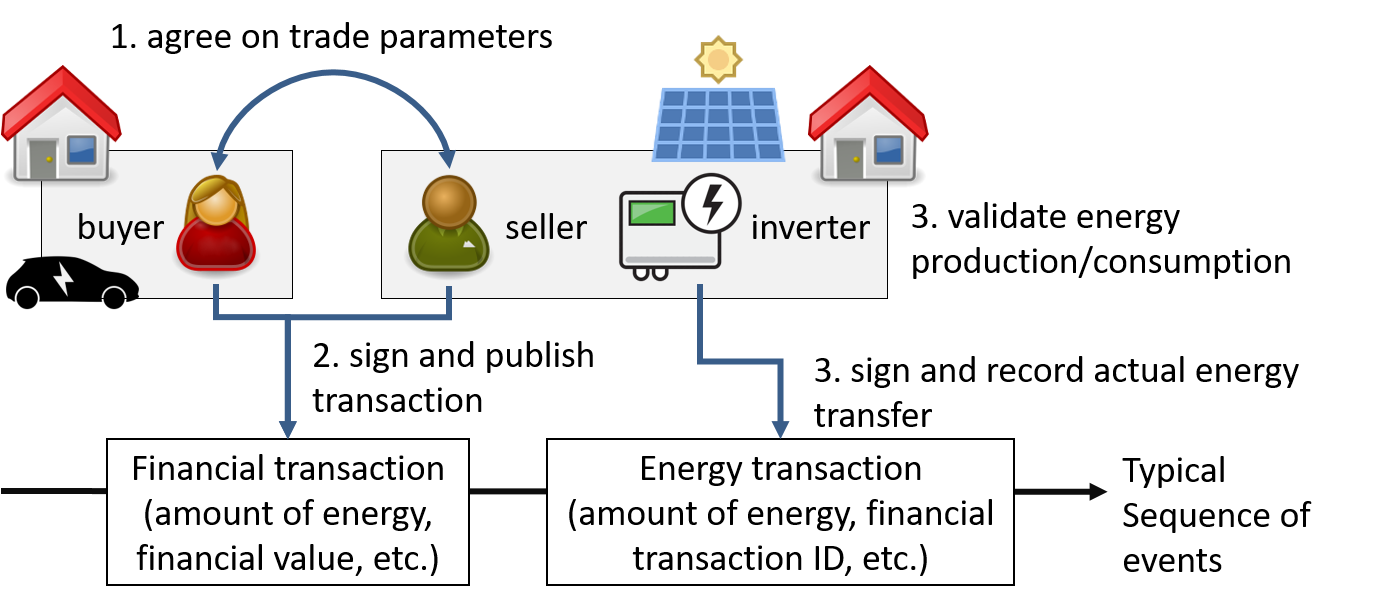
\includegraphics[width=0.5\textwidth]{diagrams/TE.png}
% \caption{A conceptual sequence of activities in a transactive energy system.  %The buyer and seller agree on the trading terms. Then, they do the actual energy transaction.
% %which must be validated.
% %Thereafter, the financial assets are transferred.
% %The red arrows show off-block chain communication and blue arrows show transactions on block-chain. Producers and consumers request the DSO to allocate the energy production and consumption assets to blockchain. The consumers receive asynchronous notification about offers from producers. Thereafter, they can finalize transaction. The energy transfer happens at a later time and is also recorded in the chain. Financial transactions are also done on the blockchain. These financial transactions are later tallied with the energy transactions.\Abhishek{Aron Lets recaption the figure
% }\label{fig:commonsequence}
% \end{figure}


%\AronC{In the problem formulation, we use ``participants'' to refer to all market participants, including the DSO.}. In this formulation, we ignore reactive power.





% \subsection{Transactive Energy Workflow}


% \label{sec:petra}
% %\textcolor{red}{There will be a figure here.}

% \Abhishek{This section should describe a typical transactive energy workflow}
% \AronC{In that case, we could keep Fig.~\ref{fig:petrasequence} and present it as an illustration of a typical workflow.}







%The key aspect of this pattern is the tight integration of distributed  messaging patterns between actors and the blockchain-based communication network used for transferring transactional information. For example, in the transactive energy domain,  
%\Karla{Unfinished sentence}

% In  \cite{Laszka17}, we introduced the key concept of privacy-preserving energy transactions where a consumer selects the producers to trade with. In this basic sequence, the smart contract is  responsible for keeping track of the energy and financial assets enabling producers to post trade offers and exchange assets when a consumer decides to accept. PETra uses quantized energy asset tokens
% %\footnote{There are two kinds of energy tokens: Energy Production Asset and Energy Consumption Asset. Token attributes include power and time interval for which the token is valid.} 
% that can represent the non-negative amount of power to be produced or consumed (for example, measured in watts),  the time interval in which energy is to be produced (or consumed), and the  last time interval in which energy is to be produced (or consumed) (Figure \ref{fig:petrasequence} describes the full sequence of activity)\AronC{Figure \ref{fig:petrasequence} is not an accurate representation of PETra or the Middleware'17 sequence!}.\AbhishekC{Aron please remove this figure and update the sequence} These assets are withdrawn and submitted to anonymized accounts on behalf of prosumers by the DSO, who is also responsible for validating that the specific prosumer has the  energy capacity for feasible trades given the assets. Once the DSO posts the assets into the blockchain, prosumers can trade between themselves using these quantized assets and anonymized addresses, hiding their identity from each other. The DSO is also responsible for releasing and managing the transfer of currencies, which are represented by financial assets, which is  simply an unsigned integer value, denominated in a fiat currency. In this workflow, there are both on- and off-blockchain communications between DSO and prosumer. The off-blockchain communication is required to request the transfer of assets. On-blockchain communication occurs via filters that track the posting of assets. Similarly, prosumers also communicate which each other via blockchain to indicate when an offer has been posted and when a transaction has cleared. 

% \Abhishek{We need to introduce  the energy trading problem using this figure}

%\item Participates in a wholesale market to supply residual demand

% \begin{itemize}
% \item 
% %\item We consider a microgrid consisting of a set 


% \Abhishek{We assume that the DSO manages the necessary reactive power balance via local capacitor banks in this setup. Note that in a generalized problem, we will have to consider that the prosumers can control reactive power generation via power electronics. A related paper is \\cite\{Kotur2016\}}
% \item  The limit is specified in terms of integers (smart contract cannot do floats). 
% %\Karla{Consider the alternative formulation above}

% %\item Feeder $f$ has a maximal carrying capacity of $C_f$ Watts. This carrying capacity is enforced using a over-current protection unit that sets the limit of total current flowing through the feeder. The limit is specified in terms of Integers (smart contract cannot do floats). 
% \Karla{We need to make sure we are consistent about the meaning of $C_f$ - power or energy? We should make sure we are consistent with the literature}
% \Abhishek{The feeders are rated with instantaneous power.}
% \Aron{I would avoid mentioning implementation details here (e.g., representing certain numbers as integers due to lack of built-in support for floats).
% Regarding the energy/power question, they are interchangeable as long as we fix the time interval (which we do in most cases).}

% \item There is a DSO that operates the microgrid and has the following abilities and responsibilities:
% \begin{itemize}
% \item Controls the participants' access to the local market
% \item Participates in the futures market to shape the prosumers' consumption and production
% \item Participates in a wholesale market to supply residual demand
% %\item Incentivizes appropriate levels of trade activity in order to shape the overall microgrid load profile
% %\Karla{@Abhishek: does DSO do this by setting prices alone? What are it's ``acutators'' in the market? Do we want to consider some sort of load curtailment scheme in addition to the market?}
% %\Abhishek{I dont think we are talking about incentives in this paper. So, we can ignore this. The optimization problem itself includes a term for matching the load profile.}
% \end{itemize}
% \end{itemize}

%\subsection{Requirement Analysis}\label{sec:requirements}
%\Abhishek{I copied this over from Middleware paper. We need to keep the things that are required for this paper}
%We aim to design a TMP that can accommodate a number of different P2P trading scenarios. In this section we describe these scenarios, and a set of system requirements that a TMP would need to meet. 


%There are a number of commercially available products that enable the real-time management and operation of microgrid distribution systems such as those considered here. For example, the Siemens DERMS suite includes Spectrum Power \cite{SpectrumPower}, which allows utilities and DSOs to optimize and control the operation of DERs on a distribution microgrid. Such products are appropriate for systems involving utility-owned DER and/or prosumer-owned DERs that are operated by the utility under utility-run opt-in programs.
%However, in order to realize a local peer-to-peer electricity market, such products need to integrate market logic that allows participants to post offers to buy and sell electricity futures in a way that preserves both system stability and prosumer interests such as privacy. From the utilities' or DSO's perspective, such extensions to existing products would enable new business models and the availability of fine-grained ancillary services. 

%In this paper, we consider problem settings in which the distribution system operator (DSO) controls the participants' access to the local market and also participates in the futures market to shape the prosumers' consumption and production. Additionally, the DSO participates in a wholesale market to provide support for any residual demand from the microgrid.



%\AbhishekC{Integrate Prior Petra Concepts}

%For example, in our prior work \cite{Laszka17} an offer consists of quantity of energy being bought or sold, the time interval in which the energy is to be produced or consumed, and a reservation price - the maximum (or respectively, minimum) price at which the buyer (or respectively, seller) is willing to trade. 
%This is done by first posting offers to sell produced energy, or offers to buy and consume energy. An offer consists of quantity of energy being bought or sold, the time interval in which the energy is to be produced or consumed, and a reservation price - the maximum (or respectively, minimum) price at which the buyer (or respectively, seller) is willing to trade. \scott{does the offer need to include when the power will be available? The time interval mentioned here sounds like the time when the offer will expire.}\Karla{@Scott, see now}%The DSO bargains on the bulk market and provides all residual supply and demand within the microgrid.  

%\Karla{I recommend describing the workflow (i.e. event sequencing) here. When is the market cleared}


\subsection{System Requirements}
\label{sec:requirements}

We now describe  requirements that  must be considered for building a decentralized Transaction Management Platform (TMP) that supports the workflow across the microgrid described above.
%consider and specify.

\subsubsection{Communication Fabric}

The first requirement is the existence of an appropriate communication and messaging architecture. The TMP must collect participants' offers and make them available to buyers and sellers, and the market algorithm must communicate clearing prices and buyer-seller matchings.
%, or other market-related signals depending on the trading scenario. 
In order to meet the operational and safety requirements described next, these messages must be reliably delivered under strict timing constraints, derived from the deadline by which a trade must clear. Moreover, the TMP must be capable of handling high volumes of micro-transactions anticipated in peer-to-peer trading scenarios.  Finally, the communication fabric must support confidentiality, integrity, and non-repudiation of transactional data.

%two important points to consider (a)  Each feeder is rated for a maximal power capacity\footnote{Physically, the capacity limit of a feeder can be enforced using an overcurrent protection unit that limits the total current flowing through the feeder.}. Therefore, it is important to ensure that local energy trade settlements involve net power production and consumption which result in instantaneous power flows that never violate this safety constraint; and (b) It is important to be able to track and validate the settlement of all trades in this market while ensuring privacy of the participants is preserved. Specifically these points 



\subsubsection{Operational Safety and Stability}

%\scottC{This section could be clearer. It's hard to tell what the actual requirements are. These should be listed then explained. I'd guess to be considered operationally safe the grid must be balanced, the hardware limits cannot be exceeded and the system must tolerate malicious or negligent behavior. Then describe each of those in more detail.}
The trading activity shall not compromise the stability of the physical system operation. For example, capacity constraints along any feeder should be respected. Specifically, each feeder is rated for a maximal power capacity.\footnote{Physically, the capacity limit of a feeder can be enforced using an overcurrent protection unit that limits the total current flowing through the feeder.} Therefore, it is important to ensure that local energy trade settlements involve power production and consumption which result in instantaneous power flows that never violate this safety constraint.
%\scottC{the congestion part is confusing. Should it say something like: "The trading activity shall not compromise the stability of the system. This can be enforced by respecting the feeder congestion constraints. Feeders are rated for a maximal power capacity ..." }

%Resiliency refers to the system's ability to react to contingencies and recover from faults. 
%Capacity constraints refer to the maximal power flow allowed on a transmission line. %The satisfaction of capacity constraints requires assurance that malicious or negligent trading activity is discouraged.
%by using active mechanisms such as congestion pricing and reputation scores. \Abhishek{Need to clarify in the implementation that this is done at coarse-level so that anonymity is not affected} \Aron{Since we don't actually have a reputation system in our implementation, we could omit this for the sake of simplicity} 
%Negligent trading may include producers who commit to a certain production level and fail to deliver. Transactional security means that the execution of contractual obligations among all participants, including the DSO, is guaranteed.
%Finally, the TMP should have provisions for preventing or detecting negligent or malicious interference with smart meters - i.e. the adversarial or natural attacks against the interface between the physical world and the blockchain; data logged shall be securely communicated to the DSO and requests made by the meter on behalf of the prosumer shall be accurately recorded on the blockchain. 

\subsubsection{Market Security and Efficiency}

The TMP shall include provisions for ensuring the protection of prosumer interests, as well as those of the DSO. Prosumer interests include being billed correctly based on energy prices set by the market and the measurements made by the smart meters. In the context of grid-connected microgrids, the system should match supply and demand as closely as possible, while respecting safety constraints. Therefore, the TMP should  aim to maximize the amount of energy traded.

%s market efficiency by maximizing transaction volume. %Additionally, it is important to ensure all prosumers will be allowed to participate in the market fairly \scott{what does it mean to participate fairly?}.
%, and being billed fairly by the DSO.


\subsubsection{Privacy}

Information such as the amount of energy produced, consumed, bought, or sold by any prosumer should be available only to the Distribution System Operator\footnote{We are building a trading system in this paper and do not explicitly address the problem of billing. However, multiple billing approaches may be implemented on top of the blockchain, some of which could provide a very high level of privacy. This will be part of our future work.}. All bids and asks, and the matching thereof, should remain anonymous to the other participants. A participant's energy usage patterns and personal information, such as financial standing, shall not be inferable from the participant's trading activity. For example, inference of energy usage patterns can be exploited by inferring the presence or absence of a person in their home.





%\scottC{does the DSO only know the total consumption for the billing cycle, or do they have all the detailed information?} \AronC{We are building the trading system, billing is on top of that, so we do not address this question in this paper. We could add a sentence saying that multiple billing approaches may be implemented on top of the blockchain, some of which could provide a very high level of privacy.} and the essential market functions of the TMP.





\section{Analysis of State of the Art}
\label{sec:related}
%\AbhishekC{We need to describe and update the state of the art by a deep dive on how transactive energy has been implemented till now - the current related research is not going into depth}



%\textbf{Transaction Management Platforms (TMP) for Smart grid} 
Implementing a Transaction Management Platforms (TMP) requires a communication architecture, as well as trading mechanisms that provide the capability to match the bids and asks.  Blockchain-based solutions have the potential to enable large-scale energy trading based on distributed consensus systems. However, popular blockchain solutions, such as Bitcoin \cite{Satoshi} and Ethereum \cite{buterin2013ethereum}, suffer from design limitations that prevent their direct application to validating energy trades. This is primarily due to the lack of additional constraints and checks required, beyond just the transactional integrity check provided by proof-of-work algorithms.
%In particular, their transaction-confirmation time is relatively slow and variable.
%proof-of-work algorithm\AronC{Our implementation also uses proof-of-work, so I would be careful with dissing it like this}.
%\Aron{What do we mean by dependence on ``on-the-blockchain communication?'' Where was the quote taken from?} dependence on ``on-the blockchain communication.'' 

For example, Aitzhan and Svetinovic implemented a proof-of-concept platform for decentralized smart grid energy trading using blockchains, but their system is based on proof-of-work consensus, and they do not consider grid control and stability, or scalability~\cite{aitzhan2016security}. Additionally, there is still the problem of privacy---all transactions in these systems are  public \cite{kosba2016hawk}. 

Most works discussing privacy look at it from the context of smart meters. McDaniel and McLaughlin discuss the
privacy concerns of energy usage profiling, which smart grids could
potentially enable~\cite{mcdaniel2009security}. Efthymiou and Kalogridis describe a method for securely anonymizing frequent electrical metering data sent by a smart
meter~\cite{efthymiou2010smart} by using a third party escrow mechanism. Tan et
al.\ study privacy in a smart metering system from an information
theoretic perspective in the presence of energy harvesting and storage
units~\cite{tan2013increasing}. They show that energy harvesting
provides increased privacy by diversifying the energy source, while a
storage device can be used to increase both energy efficiency and
privacy. However, the transaction data provides more fine-grained information than the smart meter usage patterns \cite{Privacy2017}. 

Majumder et al.\ present an iterative double auction trading mechanism that preserves the participants' privacy~\cite{majumder_efficient_2014}. However, the privacy property pertains to the participants' utility function models, not their identities. 
%In \cite{majumder_efficient_2014} Majumder et al, present an iterative double auction which aims to maximize agent utilities and overall social welfare. They also claim to maintain the privacy of users, however the objective of their approach is to incentivize participants to share personal information and that privacy is preserved because they do not relinquish all of their data. Additionally they assume  there are many participants that have limited computational power. Second, they do not consider the safety constraints of the feeders. Finally, they do not have protection against malicious participants.

Existing energy trading markets, such as the European Energy Exchange \cite{EPEX_SPOT_operation} and project NOBEL in Spain, employ the double-auction market mechanism \cite{Ilic12}, which can be implemented to preserve participant privacy. However, typical exchange implementations involve centralized database architectures prone to single points of failure.
 
%Zhang et al., also present a TMP, recognizing that transactive energy systems are vulnerable to attack due to the public transactions, and grid control over the Internet~\cite{zhang_cyber_????}. \Karla{Please fix reference!} In their work they develop a simulation architecture on top of the open source TESP (Transactive Energy Simulation Platform) in order to analyze the effects of two types of attacks (malicious bid price and quantity) on the double-auction market they implemented. This data allowed them to use a deep learning approach called deep stacked autoencoder to train a classifier to identify the two attacks. They are able to do this using the raw sensor data.

Faqiry and Das present an auction mechanism for maximizing social welfare of buyers and sellers (if the supply is small)~\cite{faqiry_transactive_2016}. Their approach also provides some privacy meaning that a participant does not reveal their utility function. By constricting the buyers' utility functions to be convex, the social welfare objective function is maximized when the micro-grid controller objective function, whose goal is to pair as maximize the power sold, is maximized. In the later part of the paper, in order to make the trading fair, they consider an approach that discards the privacy maintained during the first phase. In their work, there is no mechanism to check whether the buyer can produce the power they claim they can supply, which could result in instability. The authors also mention in passing that their approach can be implemented as a distributed algorithm, but this was not carried out. 

In contrast, the work presented in this paper is a distributed systems mechanism that considers the problem of a broader definition of privacy, safety, and protection from malicious actors as a combined problem.
%\AbhishekC{we need to reprhase our contributions and requirements here again and show why the state of the art has not yet solved the problem.}
% The work presewnted in this paper extends these works by  (1) leveraging a decentralized computation fabric provided by smart homes in the community,
% %\footnote{We demonstrate the execution on a network of virtual machines in this paper.} 
% (2) addressing the privacy
% threat posed by trading using a novel trading sequence implementation, (3) showing how partial trades can be fulfilled, and (4) designing and implementing the distributed


% and (4) using off-blockchain communication primitives provided by the distributed application management platform RIAPS. While the conceptual design of PETra was presented in \cite{Laszka17}, this paper describes the revised protocol and the trading algorithm, and presents the implementation results. 
% %This work is closely related to \cite{kosba2016hawk} .... \Abhishek{Todo:Write about Hawk}
% on, as well as support for deploying algorithms on devices across the network\footnote{RIAPS uses ZeroMQ \cite{hintjens2010zeromq}, and Cap'n Proto \cite{varda2015cap}, to manage the communication layer.} and solves problems collaboratively by providing micro-second level time synchronization \cite{riaps2}, failure based reconfiguration \cite{dubey2017resilience}, and group creation and coordination services (still under active development), in addition to the services described in \cite{LeeNiddodiSrivastavaBakken2016}. It is capable of handling different communication and running implemented algorithms in real-time.


% \Karla{this section is a duplicate of the previous}
% \color{red}
% \textbf{Transaction Management Platforms (TMP) for Smart grid} 
% TMP require communication, as well as trading mechanisms that provide the capability to match the bids and asks. Additionally, they must provide fairness and integrity assurances.  Blockchain based solutions have the potential to enable large-scale energy trading based on distributed consensus systems. However, popular blockchain solutions, such as Bitcoin \cite{Satoshi} and Ethereum \cite{buterin2013ethereum} suffer from design limitations that prevent their direct application to validating energy trades. In particular, their transaction-confirmation time is relatively slow and variable, primarily due to the proof-of-work algorithm and most of the communication occurring via the ledger.
% %\Aron{What do we mean by dependence on ``on-the-blockchain communication?'' Where was the quote taken from?} dependence on ``on-the blockchain communication.'' 
% For example, Aitzhan and Svetinovic implemented a proof-of-concept platform for decentralized smart grid energy trading using blockchains, but their system is based on proof-of-work consensus, and they do not consider grid control and stability, or scalability~\cite{aitzhan2016security}. Additionally, there is the problem of privacy - all transactions in these systems are  public \cite{kosba2016hawk}. 

% Most works in this area have focused on the privacy issue from the context of smart meters. McDaniel and McLaughlin discuss the
% privacy concerns of energy usage profiling, which smart grids could
% potentially enable~\cite{mcdaniel2009security}. Efthymiou and Kalogridis describe a method for securely anonymizing frequent electrical metering data sent by a smart
% meter~\cite{efthymiou2010smart} by using a third party escrow mechanism. Tan et
% al.\ study privacy in a smart metering system from an information
% theoretic perspective in the presence of energy harvesting and storage
% units~\cite{tan2013increasing}. They show that energy harvesting
% provides increased privacy by diversifying the energy source, while a
% storage device can be used to increase both energy efficiency and
% privacy. However, the transaction data provides more fine-grained information than the smart meter usage patterns \cite{Privacy2017}. 

% PETra extends these works by (1) leveraging a decentralized computation fabric provided by smart homes in the community,
% %\footnote{We demonstrate the execution on a network of virtual machines in this paper.} 
% (2) addressing the privacy
% threat posed by trading using a novel trading sequence implementation, (3) showing how partial trades can be fulfilled, and (4) using off-blockchain communication primitives provided by the distributed application management platform RIAPS. While the conceptual design of PETra was presented in \cite{Laszka17}, this paper describes the revised protocol and the trading algorithm, and presents the implementation results. 
% %This work is closely related to \cite{kosba2016hawk} .... \Abhishek{Todo:Write about Hawk}

% \color{black}
